\documentclass[11pt,a4paper,BCOR12mm, headexclude, footexclude, twoside, openright]{scrartcl} 
\usepackage[scaled]{helvet}
\usepackage[british]{babel}
\usepackage[utf8]{inputenc}
\usepackage[T1]{fontenc}
\usepackage{fancyhdr}
\usepackage{lastpage}
\usepackage{ifthen}
\usepackage{amsmath,amsfonts,amsthm}
\usepackage{sfmath}
\usepackage{makecell}
\usepackage{booktabs}
\usepackage{sectsty}
\usepackage{xcolor}
\usepackage{tikz}
%\KOMAoptions{optionenliste}
%\KOMAoptions{Option}{Werteliste}

\newcommand*{\TakeFourierOrnament}[1]{{%
\fontencoding{U}\fontfamily{futs}\selectfont\char#1}}
\newcommand*{\danger}{\TakeFourierOrnament{66}}
\addtokomafont{caption}{\small}
%\setkomafont{descriptionlabel}{\normalfont
%	\bfseries}
\setkomafont{captionlabel}{\normalfont
	\bfseries}
\let\oldtabular\tabular
\renewcommand{\tabular}{\sffamily\oldtabular}
\KOMAoptions{abstract=true}
%\setkomafont{footnote}{\sffamily}
%\KOMAoptions{twoside=true}
%\KOMAoptions{headsepline=true}
%\KOMAoptions{footsepline=true}
\renewcommand\familydefault{\sfdefault}
\renewcommand{\arraystretch}{1.1}
\newcommand{\horrule}[1]{\rule{\linewidth}{#1}}
\setlength{\textheight}{230mm}
\allsectionsfont{\centering \normalfont\scshape}
\let\tmp\oddsidemargin
\let\oddsidemargin\evensidemargin
\let\evensidemargin\tmp
\reversemarginpar

\numberwithin{equation}{section} % Number equations within sections (i.e. 1.1, 1.2, 2.1, 2.2 instead of 1, 2, 3, 4)
\numberwithin{figure}{section} % Number figures within sections (i.e. 1.1, 1.2, 2.1, 2.2 instead of 1, 2, 3, 4)
\numberwithin{table}{section} % Number tables within sections (i.e. 1.1, 1.2, 2.1, 2.2 instead of 1, 2, 3, 4)

\setlength\parindent{0pt}

\definecolor{CFFCC00}{HTML}{FFCC00}
\definecolor{C000000}{HTML}{000000}
\definecolor{CFFFFFF}{HTML}{FFFFFF}
\definecolor{C00FF00}{HTML}{00FF00}
\begin{document}
%\sffamily
\fancypagestyle{plain}
{%
  \renewcommand{\headrulewidth}{0pt}%
  \renewcommand{\footrulewidth}{0.5pt}
  \fancyhf{}%
  \fancyfoot[R]{\emph{\footnotesize Page \thepage\ of \pageref{LastPage}}}%
  \fancyfoot[C]{\emph{\footnotesize Samy Aittahar}}%
}

\thispagestyle{plain}

\titlehead
{
	University of Liège\hfill
    INFO8006%
}
\subject{\vspace{-1ex} \horrule{2pt}\\[0.15cm] {\textsc{\texttt{Introduction to AI}}}}
\title{Assignment 1}
\subtitle{\textsc{\texttt{The AI Sandbox}}\\\horrule{2pt}\\[0.5cm]}
\author{\bfseries{Samy Aittahar}\vspace{-2ex}}
\date{\begin{tabular}{cc}
  \textsc{Date:}& \textsc{\emph{\today}}
\end{tabular}}
\maketitle

%\begin{abstract}
%\end{abstract}

%--------------------------------------------

\section{Pratical Informations}
\begin{itemize}
	\item Teaching Assistant : Samy Aittahar ;
    \item saittahar@ulg.ac.be, office I-136 (Montefiore Institute, 1st floor) ;
    \item Format : Exercises, two big projects (Tic Tac Toe variant and Ms Pac Man, modalities to come soon).

\end{itemize}

\section{Basic search}
\begin{center}
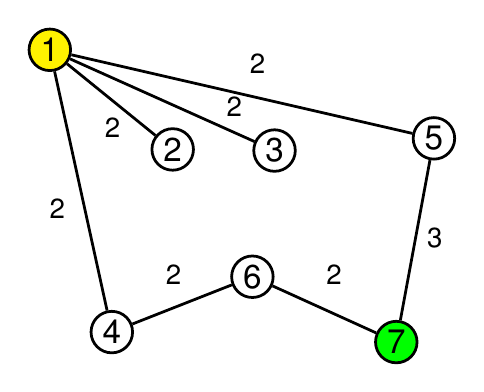
\begin{tikzpicture}[inner sep=0pt,scale=0.4]
\node (n0) [minimum height=15.0pt, minimum width=15.0pt,at={(514pt,-187pt)}, fill=yellow, draw, line width=1.0pt,align=center,text width=11.634765625,font=\fontfamily{phv}\fontsize{12}{13}\selectfont, shape=circle] {1};
\node (n1) [minimum height=15.0pt, minimum width=15.0pt,at={(625pt,-277pt)}, fill=CFFFFFF, draw, line width=1.0pt,align=center,text width=11.634765625,font=\fontfamily{phv}\fontsize{12}{13}\selectfont, shape=circle] {2};
\node (n2) [minimum height=15.0pt, minimum width=15.0pt,at={(717pt,-278pt)}, fill=CFFFFFF, draw, line width=1.0pt,align=center,text width=11.634765625,font=\fontfamily{phv}\fontsize{12}{13}\selectfont, shape=circle] {3};
\node (n3) [minimum height=15.0pt, minimum width=15.0pt,at={(861pt,-267pt)}, fill=CFFFFFF, draw, line width=1.0pt,align=center,text width=11.634765625,font=\fontfamily{phv}\fontsize{12}{13}\selectfont, shape=circle] {5};
\node (n4) [minimum height=15.0pt, minimum width=15.0pt,at={(570pt,-442pt)}, fill=CFFFFFF, draw, line width=1.0pt,align=center,text width=11.634765625,font=\fontfamily{phv}\fontsize{12}{13}\selectfont, shape=circle] {4};
\node (n5) [minimum height=15.0pt, minimum width=15.0pt,at={(697pt,-392pt)}, fill=CFFFFFF, draw, line width=1.0pt,align=center,text width=11.634765625,font=\fontfamily{phv}\fontsize{12}{13}\selectfont, shape=circle] {6};
\node (n6) [minimum height=15.0pt, minimum width=15.0pt,at={(827pt,-451pt)}, fill=green, draw, line width=1.0pt,align=center,text width=11.634765625,font=\fontfamily{phv}\fontsize{12}{13}\selectfont, shape=circle] {7};
\node (n01) [minimum height=15.0pt, minimum width=15.0pt,at={(570pt,-257pt)}, align=center,text width=5,font=\fontfamily{phv}\fontsize{10}{11}\selectfont] {2};
\node (n02) [minimum height=15.0pt, minimum width=15.0pt,at={(680pt,-238pt)}, align=center,text width=5,font=\fontfamily{phv}\fontsize{10}{11}\selectfont] {2};
\node (n03) [minimum height=15.0pt, minimum width=15.0pt,at={(701pt,-200pt)}, align=center,text width=5,font=\fontfamily{phv}\fontsize{10}{11}\selectfont] {2};
\node (n04) [minimum height=15.0pt, minimum width=15.0pt,at={(520pt,-331pt)}, align=center,text width=5,font=\fontfamily{phv}\fontsize{10}{11}\selectfont] {2};
\node (n36) [minimum height=15.0pt, minimum width=15.0pt,at={(861pt,-357pt)}, align=center,text width=5,font=\fontfamily{phv}\fontsize{10}{11}\selectfont] {3};
\node (n45) [minimum height=15.0pt, minimum width=15.0pt,at={(625pt,-390pt)}, align=center,text width=5,font=\fontfamily{phv}\fontsize{10}{11}\selectfont] {2};
\node (n56) [minimum height=15.0pt, minimum width=15.0pt,at={(770pt,-390pt)}, align=center,text width=5,font=\fontfamily{phv}\fontsize{10}{11}\selectfont] {2};
\path [-,line width=1.0pt,draw,](n0)--(n4);
\path [-,line width=1.0pt,draw,](n0)--(n1);
\path [-,line width=1.0pt,draw,](n0)--(n2);
\path [-,line width=1.0pt,draw,](n0)--(n3);
\path [-,line width=1.0pt,draw,](n4)--(n5);
\path [-,line width=1.0pt,draw,](n5)--(n6);
\path [-,line width=1.0pt,draw,](n3)--(n6);
\end{tikzpicture}
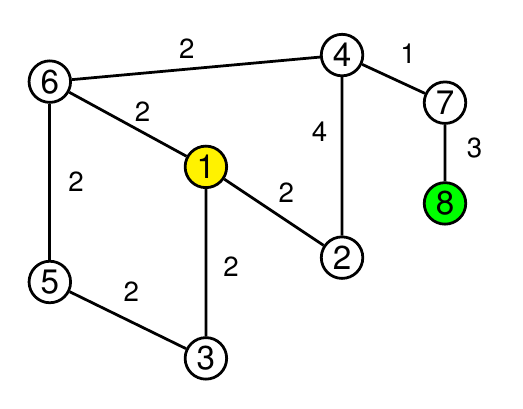
\begin{tikzpicture}[inner sep=0pt,scale=0.4]
\node (n0) [minimum height=15.0pt, minimum width=15.0pt,at={(518pt,-187pt)}, fill=yellow, draw, line width=1.0pt,align=center,text width=11.634765625,font=\fontfamily{phv}\fontsize{12}{13}\selectfont, shape=circle] {1};
\node (n1) [minimum height=15.0pt, minimum width=15.0pt,at={(518pt,-360pt)}, fill=CFFFFFF, draw, line width=1.0pt,align=center,text width=11.634765625,font=\fontfamily{phv}\fontsize{12}{13}\selectfont, shape=circle] {3};
\node (n2) [minimum height=15.0pt, minimum width=15.0pt,at={(377pt,-110pt)}, fill=CFFFFFF, draw, line width=1.0pt,align=center,text width=11.634765625,font=\fontfamily{phv}\fontsize{12}{13}\selectfont, shape=circle] {6};
\node (n3) [minimum height=15.0pt, minimum width=15.0pt,at={(377pt,-291pt)}, fill=CFFFFFF, draw, line width=1.0pt,align=center,text width=11.634765625,font=\fontfamily{phv}\fontsize{12}{13}\selectfont, shape=circle] {5};
\node (n4) [minimum height=15.0pt, minimum width=15.0pt,at={(641pt,-86pt)}, fill=CFFFFFF, draw, line width=1.0pt,align=center,text width=11.634765625,font=\fontfamily{phv}\fontsize{12}{13}\selectfont, shape=circle] {4};
\node (n5) [minimum height=15.0pt, minimum width=15.0pt,at={(641pt,-269pt)}, fill=CFFFFFF, draw, line width=1.0pt,align=center,text width=11.634765625,font=\fontfamily{phv}\fontsize{12}{13}\selectfont, shape=circle] {2};
\node (n6) [minimum height=15.0pt, minimum width=15.0pt,at={(734pt,-129pt)}, fill=CFFFFFF, draw, line width=1.0pt,align=center,text width=11.634765625,font=\fontfamily{phv}\fontsize{12}{13}\selectfont, shape=circle] {7};
\node (n7) [minimum height=15.0pt, minimum width=15.0pt,at={(734pt,-220pt)}, fill=green, draw, line width=1.0pt,align=center,text width=11.634765625,font=\fontfamily{phv}\fontsize{12}{13}\selectfont, shape=circle] {8};

\node (n01) [minimum height=15.0pt, minimum width=15.0pt,at={(540pt,-277pt)}, align=center,text width=5,font=\fontfamily{phv}\fontsize{10}{11}\selectfont] {2};
\node (n02) [minimum height=15.0pt, minimum width=15.0pt,at={(460pt,-137pt)}, align=center,text width=5,font=\fontfamily{phv}\fontsize{10}{11}\selectfont] {2};
\node (n05) [minimum height=15.0pt, minimum width=15.0pt,at={(590pt,-210pt)}, align=center,text width=5,font=\fontfamily{phv}\fontsize{10}{11}\selectfont] {2};
\node (n13) [minimum height=15.0pt, minimum width=15.0pt,at={(450pt,-300pt)}, align=center,text width=5,font=\fontfamily{phv}\fontsize{10}{11}\selectfont] {2};
\node (n23) [minimum height=15.0pt, minimum width=15.0pt,at={(400pt,-200pt)}, align=center,text width=5,font=\fontfamily{phv}\fontsize{10}{11}\selectfont] {2};
\node (n24) [minimum height=15.0pt, minimum width=15.0pt,at={(500pt,-80pt)}, align=center,text width=5,font=\fontfamily{phv}\fontsize{10}{11}\selectfont] {2};
\node (n54) [minimum height=15.0pt, minimum width=15.0pt,at={(620pt,-155pt)}, align=center,text width=5,font=\fontfamily{phv}\fontsize{10}{11}\selectfont] {4};
\node (n46) [minimum height=15.0pt, minimum width=15.0pt,at={(700pt,-85pt)}, align=center,text width=5,font=\fontfamily{phv}\fontsize{10}{11}\selectfont] {1};
\node (n68) [minimum height=15.0pt, minimum width=15.0pt,at={(760pt,-170pt)}, align=center,text width=5,font=\fontfamily{phv}\fontsize{10}{11}\selectfont] {3};


\path [-,line width=1.0pt,draw,](n2)--(n0);
\path [-,line width=1.0pt,draw,](n2)--(n3);
\path [-,line width=1.0pt,draw,](n3)--(n1);
\path [-,line width=1.0pt,draw,](n1)--(n0);
\path [-,line width=1.0pt,draw,](n0)--(n5);
\path [-,line width=1.0pt,draw,](n5)--(n4);
\path [-,line width=1.0pt,draw,](n4)--(n6);
\path [-,line width=1.0pt,draw,](n2)--(n4);
\path [-,line width=1.0pt,draw,](n6)--(n7);
\end{tikzpicture}

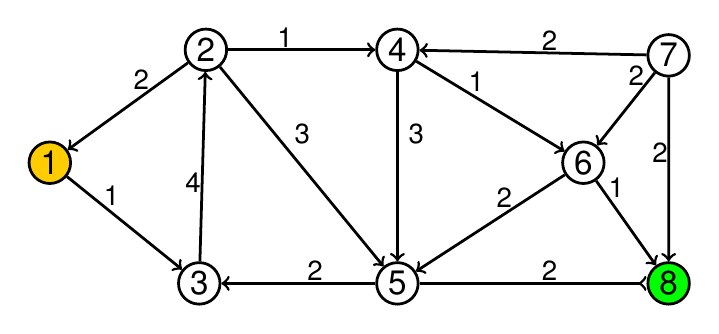
\begin{tikzpicture}[inner sep=0pt,scale=0.4]
\node (n0) [minimum height=15.0pt, minimum width=15.0pt,at={(514pt,-187pt)}, fill=CFFCC00, draw, line width=1.0pt,align=center,text width=11.634765625,font=\fontfamily{phv}\fontsize{12}{13}\selectfont, shape=circle] {1};
\node (n1) [minimum height=15.0pt, minimum width=15.0pt,at={(655pt,-85pt)}, fill=CFFFFFF, draw, line width=1.0pt,align=center,text width=11.634765625,font=\fontfamily{phv}\fontsize{12}{13}\selectfont, shape=circle] {2};
\node (n2) [minimum height=15.0pt, minimum width=15.0pt,at={(649pt,-296pt)}, fill=CFFFFFF, draw, line width=1.0pt,align=center,text width=11.634765625,font=\fontfamily{phv}\fontsize{12}{13}\selectfont, shape=circle] {3};
\node (n3) [minimum height=15.0pt, minimum width=15.0pt,at={(828pt,-85pt)}, fill=CFFFFFF, draw, line width=1.0pt,align=center,text width=11.634765625,font=\fontfamily{phv}\fontsize{12}{13}\selectfont, shape=circle] {4};
\node (n4) [minimum height=15.0pt, minimum width=15.0pt,at={(828pt,-296pt)}, fill=CFFFFFF, draw, line width=1.0pt,align=center,text width=11.634765625,font=\fontfamily{phv}\fontsize{12}{13}\selectfont, shape=circle] {5};
\node (n5) [minimum height=15.0pt, minimum width=15.0pt,at={(996pt,-187pt)}, fill=CFFFFFF, draw, line width=1.0pt,align=center,text width=11.634765625,font=\fontfamily{phv}\fontsize{12}{13}\selectfont, shape=circle] {6};
\node (n6) [minimum height=15.0pt, minimum width=15.0pt,at={(1073pt,-90pt)}, fill=CFFFFFF, draw, line width=1.0pt,align=center,text width=11.634765625,font=\fontfamily{phv}\fontsize{12}{13}\selectfont, shape=circle] {7};
\node (n7) [minimum height=15.0pt, minimum width=15.0pt,at={(1073pt,-296pt)}, fill=C00FF00, draw, line width=1.0pt,align=center,text width=11.634765625,font=\fontfamily{phv}\fontsize{12}{13}\selectfont, shape=circle] {8};


\path [->,line width=1.0pt,draw,](n1)--(n0);
\path (n1) ++(-58.3466186523438pt,-27.0155116953748pt)node[align=center,text width=11.634765625,font=\fontfamily{phv}\fontsize{10}{11}\selectfont]{2};

\path [->,line width=1.0pt,draw,](n0)--(n2);
\path (n0) ++(55.8292846679688pt,-29.3955770987051pt)node[align=center,text width=11.634765625,font=\fontfamily{phv}\fontsize{10}{11}\selectfont]{1};



\path [->,line width=1.0pt,draw,](n1)--(n3);
\path (n1) ++(71.5pt,10.984375pt)node[align=center,text width=11.634765625,font=\fontfamily{phv}\fontsize{10}{11}\selectfont]{1};

\path [->,line width=1.0pt,draw,](n2)--(n1);
\path (n2) ++(-5.499254271882364pt,90.5060729980469pt)node[align=center,text width=11.634765625,font=\fontfamily{phv}\fontsize{10}{11}\selectfont]{4};

\path [->,line width=1.0pt,draw,](n4)--(n2);
\path (n4) ++(-74.5pt,10.984375pt)node[align=center,text width=11.634765625,font=\fontfamily{phv}\fontsize{10}{11}\selectfont]{2};

\path [->,line width=1.0pt,draw,](n1)--(n4);
\path (n1) ++(86.9894409179688pt,-75.8208795889265pt)node[align=center,text width=11.634765625,font=\fontfamily{phv}\fontsize{10}{11}\selectfont]{3};

\path [->,line width=1.0pt,draw,](n3)--(n4);
\path (n3) ++(16.9894409179688pt,-75.8208795889265pt)node[align=center,text width=11.634765625,font=\fontfamily{phv}\fontsize{10}{11}\selectfont]{3};

\path [->,line width=1.0pt,draw,](n6)--(n7);
\path (n6) ++(-7.8173828125pt,-88pt)node[align=center,text width=11.634765625,font=\fontfamily{phv}\fontsize{10}{11}\selectfont]{2};

\path [>-,line width=1.0pt,draw,](n7)--(n4);
\path (n7) ++(-107.5pt,10.984375pt)node[align=center,text width=11.634765625,font=\fontfamily{phv}\fontsize{10}{11}\selectfont]{2};

\path [->,line width=1.0pt,draw,](n5)--(n4);
\path (n5) ++(-71.41650390625pt,-31.5769602457682pt)node[align=center,text width=11.634765625,font=\fontfamily{phv}\fontsize{10}{11}\selectfont]{2};

\path [->,line width=1.0pt,draw,](n6)--(n5);
\path (n6) ++(-29.1739501953125pt,-18.4388358376243pt)node[align=center,text width=11.634765625,font=\fontfamily{phv}\fontsize{10}{11}\selectfont]{2};

\path [->,line width=1.0pt,draw,](n3)--(n5);
\path (n3) ++(71.1781616210938pt,-28.6989669799805pt)node[align=center,text width=11.634765625,font=\fontfamily{phv}\fontsize{10}{11}\selectfont]{1};

\path [->,line width=1.0pt,draw,](n6)--(n3);
\path (n6) ++(-107.503173828125pt,13.2970363071987pt)node[align=center,text width=11.634765625,font=\fontfamily{phv}\fontsize{10}{11}\selectfont]{2};

\path [->,line width=1.0pt,draw,](n5)--(n7);
\path (n5) ++(29.8453369140625pt,-23.0292247425426pt)node[align=center,text width=11.634765625,font=\fontfamily{phv}\fontsize{10}{11}\selectfont]{1};
\end{tikzpicture}
\end{center}
For each of the graphs, perform the following searches and discuss what happens : 

\begin{itemize}
	\item Depth-first search
    \item Breadth-first search
    \item Uniform cost
\end{itemize}

\danger The last one is directed ! Possible to go through an opposite direction but cost is 2x the original one\\
(At any tie, least labeled node is to be considered first. Plus, any expanded node is considered as visited)

What is common for all these methods ? What are some important properties for each of them ? Can you cite another search method you've seen, either in class or outside ?

\section{$\textnormal{Worms}^{(tm)}$ and $A^*$}
Help Glörm the Worm to reach the Bazooka as quick as possible, with $A^*$. Try a shot whether the diagonal move is allowed or not.
\begin{center}
\begin{tikzpicture}[inner sep=0pt]
\node (n0) [minimum height=30.0pt, minimum width=30.0pt,at={(510pt,-270pt)}, fill=CFFFFFF, draw, line width=1.0pt,align=center,text width=11.634765625,font=\fontfamily{phv}\fontsize{12}{13}\selectfont, shape=rectangle] {};
\node (n1) [minimum height=30.0pt, minimum width=30.0pt,at={(510pt,-300pt)}, fill=CFFFFFF, draw, line width=1.0pt,align=center,text width=11.634765625,font=\fontfamily{phv}\fontsize{12}{13}\selectfont, shape=rectangle] {};
\node (n2) [minimum height=30.0pt, minimum width=30.0pt,at={(510pt,-330pt)}, fill=CFFFFFF, draw, line width=1.0pt,align=center,text width=11.634765625,font=\fontfamily{phv}\fontsize{12}{13}\selectfont, shape=rectangle] {};
\node (n3) [minimum height=30.0pt, minimum width=30.0pt,at={(510pt,-360pt)}, fill=CFFFFFF, draw, line width=1.0pt,align=center,text width=11.634765625,font=\fontfamily{phv}\fontsize{12}{13}\selectfont, shape=rectangle] {};
\node (n4) [minimum height=30.0pt, minimum width=30.0pt,at={(540pt,-360pt)}, fill=CFFFFFF, draw, line width=1.0pt,align=center,text width=11.634765625,font=\fontfamily{phv}\fontsize{12}{13}\selectfont, shape=rectangle] {};
\node (n5) [minimum height=30.0pt, minimum width=30.0pt,at={(540pt,-330pt)}, fill=CFFFFFF, draw, line width=1.0pt,align=center,text width=11.634765625,font=\fontfamily{phv}\fontsize{12}{13}\selectfont, shape=rectangle] {};
\node (n6) [minimum height=30.0pt, minimum width=30.0pt,at={(540pt,-300pt)}, fill=CFFFFFF, draw, line width=1.0pt,align=center,text width=11.634765625,font=\fontfamily{phv}\fontsize{12}{13}\selectfont, shape=rectangle] {
\includegraphics[scale=0.07]{worms.png}};
\node (n7) [minimum height=30.0pt, minimum width=30.0pt,at={(540pt,-270pt)}, fill=CFFFFFF, draw, line width=1.0pt,align=center,text width=11.634765625,font=\fontfamily{phv}\fontsize{12}{13}\selectfont, shape=rectangle] {};
\node (n8) [minimum height=30.0pt, minimum width=30.0pt,at={(510pt,-240pt)}, fill=CFFFFFF, draw, line width=1.0pt,align=center,text width=11.634765625,font=\fontfamily{phv}\fontsize{12}{13}\selectfont, shape=rectangle] {};
\node (n9) [minimum height=30.0pt, minimum width=30.0pt,at={(540pt,-240pt)}, fill=CFFFFFF, draw, line width=1.0pt,align=center,text width=19.26953125,font=\fontfamily{phv}\fontsize{12}{13}\selectfont, shape=rectangle] {};
\node (n10) [minimum height=30.0pt, minimum width=30.0pt,at={(570pt,-240pt)}, fill=CFFFFFF, draw, line width=1.0pt,align=center,text width=19.26953125,font=\fontfamily{phv}\fontsize{12}{13}\selectfont, shape=rectangle] {};
\node (n11) [minimum height=30.0pt, minimum width=30.0pt,at={(570pt,-270pt)}, fill=CFFFFFF, draw, line width=1.0pt,align=center,text width=19.26953125,font=\fontfamily{phv}\fontsize{12}{13}\selectfont, shape=rectangle] {};
\node (n12) [minimum height=30.0pt, minimum width=30.0pt,at={(570pt,-300pt)}, fill=CFFFFFF, draw, line width=1.0pt,align=center,text width=19.26953125,font=\fontfamily{phv}\fontsize{12}{13}\selectfont, shape=rectangle] {};
\node (n13) [minimum height=30.0pt, minimum width=30.0pt,at={(570pt,-330pt)}, fill=CFFFFFF, draw, line width=1.0pt,align=center,text width=19.26953125,font=\fontfamily{phv}\fontsize{12}{13}\selectfont, shape=rectangle] {};
\node (n14) [minimum height=30.0pt, minimum width=30.0pt,at={(570pt,-360pt)}, fill=CFFFFFF, draw, line width=1.0pt,align=center,text width=19.26953125,font=\fontfamily{phv}\fontsize{12}{13}\selectfont, shape=rectangle] {};
\node (n15) [minimum height=30.0pt, minimum width=30.0pt,at={(600pt,-360pt)}, fill=CFFFFFF, draw, line width=1.0pt,align=center,text width=19.26953125,font=\fontfamily{phv}\fontsize{12}{13}\selectfont, shape=rectangle] {};
\node (n16) [minimum height=30.0pt, minimum width=30.0pt,at={(600pt,-330pt)}, fill=CFFFFFF, draw, line width=1.0pt,align=center,text width=19.26953125,font=\fontfamily{phv}\fontsize{12}{13}\selectfont, shape=rectangle] {};
\node (n17) [minimum height=30.0pt, minimum width=30.0pt,at={(600pt,-300pt)}, fill=CFFFFFF, draw, line width=1.0pt,align=center,text width=19.26953125,font=\fontfamily{phv}\fontsize{12}{13}\selectfont, shape=rectangle] {};
\node (n18) [minimum height=30.0pt, minimum width=30.0pt,at={(600pt,-270pt)}, fill=CFFFFFF, draw, line width=1.0pt,align=center,text width=19.26953125,font=\fontfamily{phv}\fontsize{12}{13}\selectfont, shape=rectangle] {};
\node (n19) [minimum height=30.0pt, minimum width=30.0pt,at={(600pt,-240pt)}, fill=CFFFFFF, draw, line width=1.0pt,align=center,text width=19.26953125,font=\fontfamily{phv}\fontsize{12}{13}\selectfont, shape=rectangle] {};
\node (n20) [minimum height=30.0pt, minimum width=30.0pt,at={(630pt,-240pt)}, fill=CFFFFFF, draw, line width=1.0pt,align=center,text width=19.26953125,font=\fontfamily{phv}\fontsize{12}{13}\selectfont, shape=rectangle] {};
\node (n21) [minimum height=30.0pt, minimum width=30.0pt,at={(660pt,-240pt)}, fill=CFFFFFF, draw, line width=1.0pt,align=center,text width=19.26953125,font=\fontfamily{phv}\fontsize{12}{13}\selectfont, shape=rectangle] {};
\node (n22) [minimum height=30.0pt, minimum width=30.0pt,at={(690pt,-240pt)}, fill=CFFFFFF, draw, line width=1.0pt,align=center,text width=19.26953125,font=\fontfamily{phv}\fontsize{12}{13}\selectfont, shape=rectangle] {};
\node (n23) [minimum height=30.0pt, minimum width=30.0pt,at={(720pt,-240pt)}, fill=CFFFFFF, draw, line width=1.0pt,align=center,text width=19.26953125,font=\fontfamily{phv}\fontsize{12}{13}\selectfont, shape=rectangle] {};
\node (n24) [minimum height=30.0pt, minimum width=30.0pt,at={(720pt,-270pt)}, fill, draw, line width=1.0pt,align=center,text width=19.26953125,font=\fontfamily{phv}\fontsize{12}{13}\selectfont, shape=rectangle] {};
\node (n25) [minimum height=30.0pt, minimum width=30.0pt,at={(720pt,-300pt)}, fill=CFFFFFF, draw, line width=1.0pt,align=center,text width=19.26953125,font=\fontfamily{phv}\fontsize{12}{13}\selectfont, shape=rectangle] {};
\node (n26) [minimum height=30.0pt, minimum width=30.0pt,at={(720pt,-330pt)}, fill, draw, line width=1.0pt,align=center,text width=19.26953125,font=\fontfamily{phv}\fontsize{12}{13}\selectfont, shape=rectangle] {};
\node (n27) [minimum height=30.0pt, minimum width=30.0pt,at={(690pt,-360pt)}, fill=CFFFFFF, draw, line width=1.0pt,align=center,text width=19.26953125,font=\fontfamily{phv}\fontsize{12}{13}\selectfont, shape=rectangle] {};
\node (n28) [minimum height=30.0pt, minimum width=30.0pt,at={(720pt,-360pt)}, fill=CFFFFFF, draw, line width=1.0pt,align=center,text width=19.26953125,font=\fontfamily{phv}\fontsize{12}{13}\selectfont, shape=rectangle] {};
\node (n29) [minimum height=30.0pt, minimum width=30.0pt,at={(690pt,-330pt)}, fill=CFFFFFF, draw, line width=1.0pt,align=center,text width=19.26953125,font=\fontfamily{phv}\fontsize{12}{13}\selectfont, shape=rectangle] {};
\node (n30) [minimum height=30.0pt, minimum width=30.0pt,at={(690pt,-300pt)}, fill=CFFFFFF, draw, line width=1.0pt,align=center,text width=19.26953125,font=\fontfamily{phv}\fontsize{12}{13}\selectfont, shape=rectangle] {};
\node (n31) [minimum height=30.0pt, minimum width=30.0pt,at={(690pt,-270pt)}, fill, draw, line width=1.0pt,align=center,text width=19.26953125,font=\fontfamily{phv}\fontsize{12}{13}\selectfont, shape=rectangle] {};
\node (n32) [minimum height=30.0pt, minimum width=30.0pt,at={(660pt,-270pt)}, fill, draw, line width=1.0pt,align=center,text width=19.26953125,font=\fontfamily{phv}\fontsize{12}{13}\selectfont, shape=rectangle] {};
\node (n33) [minimum height=30.0pt, minimum width=30.0pt,at={(630pt,-270pt)}, fill=CFFFFFF, draw, line width=1.0pt,align=center,text width=19.26953125,font=\fontfamily{phv}\fontsize{12}{13}\selectfont, shape=rectangle] {};
\node (n34) [minimum height=30.0pt, minimum width=30.0pt,at={(630pt,-300pt)}, fill, draw, line width=1.0pt,align=center,text width=19.26953125,font=\fontfamily{phv}\fontsize{12}{13}\selectfont, shape=rectangle] {};
\node (n35) [minimum height=30.0pt, minimum width=30.0pt,at={(660pt,-300pt)}, fill=CFFFFFF, draw, line width=1.0pt,align=center,text width=19.26953125,font=\fontfamily{phv}\fontsize{12}{13}\selectfont, shape=rectangle] {
\includegraphics[scale=0.2]{bazooka.png}};
\node (n36) [minimum height=30.0pt, minimum width=30.0pt,at={(660pt,-330pt)}, fill, draw, line width=1.0pt,align=center,text width=19.26953125,font=\fontfamily{phv}\fontsize{12}{13}\selectfont, shape=rectangle] {};
\node (n37) [minimum height=30.0pt, minimum width=30.0pt,at={(630pt,-330pt)}, fill, draw, line width=1.0pt,align=center,text width=19.26953125,font=\fontfamily{phv}\fontsize{12}{13}\selectfont, shape=rectangle] {};
\node (n38) [minimum height=30.0pt, minimum width=30.0pt,at={(630pt,-360pt)}, fill=CFFFFFF, draw, line width=1.0pt,align=center,text width=19.26953125,font=\fontfamily{phv}\fontsize{12}{13}\selectfont, shape=rectangle] {};
\node (n39) [minimum height=30.0pt, minimum width=30.0pt,at={(660pt,-360pt)}, fill=CFFFFFF, draw, line width=1.0pt,align=center,text width=19.26953125,font=\fontfamily{phv}\fontsize{12}{13}\selectfont, shape=rectangle] {};
\node (n40) [minimum height=30.0pt, minimum width=30.0pt,at={(750pt,-240pt)}, fill=CFFFFFF, draw, line width=1.0pt,align=center,text width=19.26953125,font=\fontfamily{phv}\fontsize{12}{13}\selectfont, shape=rectangle] {};
\node (n41) [minimum height=30.0pt, minimum width=30.0pt,at={(750pt,-270pt)}, fill=CFFFFFF, draw, line width=1.0pt,align=center,text width=19.26953125,font=\fontfamily{phv}\fontsize{12}{13}\selectfont, shape=rectangle] {};
\node (n42) [minimum height=30.0pt, minimum width=30.0pt,at={(750pt,-300pt)}, fill=CFFFFFF, draw, line width=1.0pt,align=center,text width=19.26953125,font=\fontfamily{phv}\fontsize{12}{13}\selectfont, shape=rectangle] {};
\node (n43) [minimum height=30.0pt, minimum width=30.0pt,at={(750pt,-330pt)}, fill=CFFFFFF, draw, line width=1.0pt,align=center,text width=19.26953125,font=\fontfamily{phv}\fontsize{12}{13}\selectfont, shape=rectangle] {};
\node (n44) [minimum height=30.0pt, minimum width=30.0pt,at={(750pt,-360pt)}, fill=CFFFFFF, draw, line width=1.0pt,align=center,text width=19.26953125,font=\fontfamily{phv}\fontsize{12}{13}\selectfont, shape=rectangle] {};
\end{tikzpicture}
\end{center}

\section{Safe traveling}

An assassin, a templar and the police chief have to go in a meeting to negotiate a truce (fans should have enough imagination to figure out some reasons...).\\

They travel altogether with a trouble-shooter in order to avoid a bloodbath even before they reach the meeting. Everything is working fine until they meet a river, with a boat which can contains only two persons.\\

The trouble-shooter has made his homework and knows the following facts : 

\begin{itemize}
	\item If the templar is alone with the assassin, they'll fight until death,
    \item If the assassin is alone with the police chief, he will sneakily kill him. 
\end{itemize}

(If one of them happens, there will be no truce, and consequences will follow).\\

The goal of the trouble-shooter is to bring all of them in the other side.\\

Unfortunately, the trouble-shooter did not attend this IA course and then don't know how to quickly formalize the problem and find the path which will make him accomplish his goal ! So he decided to ask the whole class to solve this issue, because the prof and the teaching assistant are too b... well, they want them to learn.\\

Fortunately, as you have been really attentive to the course, you have all the elements to represent and solve this problem. Give a try ! And don't hesitate to ask the teaching assistant if you're stuck, he's been paid for that !



%\begin{description}
%	\item[empty] ist der Seitenstil, bei dem Kopf- und Fusszeile vollständig 	leer bleiben.\marginpar[\textit{Randnotiz links}]
%	{\textit{Randnotiz rechts}}
%    \item[plain] ist der Seitenstil, bei dem keinerlei Kolumnentitel verwendet wird.
%    \item[headings] ist der Seitenstil für automatische Kolumnentitel.
%    \item[myheadings] ist der Seitenstil für manuelle Kolumnentitel.
%\end{description}



%$\mathsf{({m}^{3}/s)}$
%-------------------------------
%\begin{figure}
%	\setcapindent{-1em}
%    \fbox{\parbox{.95\linewidth}{
%    	\centering\KOMAScript}}
%	\caption{Beispiel mit teilweise hängendem Einzug ab der zweiten Zeile}
%\end{figure}

%Guten Morgen\footnote{irgend ein text\label{refnote}}\multiplefootnoteseparator\footnote{es geht noch weiter}Blabla\footref{refnote}
\end{document}